\documentclass{exercise}

\institute{Lehr- und Forschungsgebiet Kontinuumsmechanik}
\title{Übung 9}
\author{Joshua Feld, 406718}
\course{Mechanik verformbarer Körper}
\professor{Itskov}
\semester{Sommersemester 2022}
\program{CES (Bachelor)}

\begin{document}
    \maketitle
    
    
    \section*{Aufgabe 1}
    
    \begin{problem}
        Ein Balken wird in der dargestellten Weise beansprucht.
        Die Profile \(A\) - \(D\) stehen zur Verfügung.
        Berechnen Sie die maximal zu erwartenden Biegespannungen, wenn die Querschnittsfläche stets die gleiche Größe hat.
        \begin{center}
            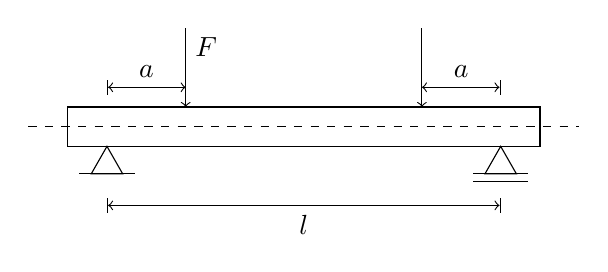
\begin{tikzpicture}
                \draw (0,0) rectangle (6,.5);
                \draw[dashed] (-.5,.25) -- (6.5,.25);
                \draw[->] (1.5,1.5) node[below right] {\(F\)} -- (1.5,.5);
                \draw[->] (4.5,1.5) -- (4.5,.5);
                \draw[|<->] (.5,.75) -- (1.5,.75) node[midway,above] {\(a\)};
                \draw[<->|] (4.5,.75) -- (5.5,.75) node[midway,above] {\(a\)};
                \draw[|<->|] (.5,-.75) -- (5.5,-.75) node[midway,below] {\(l\)};
                \draw (.3,-.35) -- (.5,0) -- (.7,-.35) -- cycle;
                \draw (.15,-.35) -- (.85,-.35);
                \draw (5.3,-.35) -- (5.5,0) -- (5.7,-.35) -- cycle;
                \draw (5.15,-.35) -- (5.85,-.35);
                \draw (5.15,-.45) -- (5.85,-.45);
            \end{tikzpicture}

            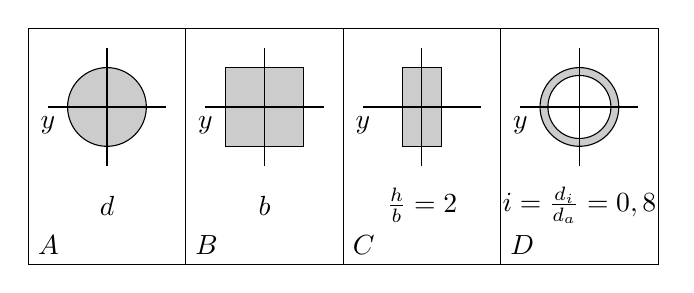
\begin{tikzpicture}
                \draw (0,0) rectangle (2,3);
                \node[anchor=south west] at (0,0) {\(A\)};
                \draw[fill=white!80!black] (1,2) circle (.5cm);
                \draw (.25,2) node[below] {\(y\)} -- (1.75,2);
                \draw (1,2.75) -- (1,1.25);
                \node at (1,.75) {\(d\)};
                \begin{scope}[shift={(2,0)}]
                    \draw (0,0) rectangle (2,3);
                    \node[anchor=south west] at (0,0) {\(B\)};
                    \draw[fill=white!80!black] (.5,1.5) rectangle (1.5,2.5);
                    \draw (.25,2) node[below] {\(y\)} -- (1.75,2);
                    \draw (1,2.75) -- (1,1.25);
                    \node at (1,.75) {\(b\)};
                \end{scope}
                \begin{scope}[shift={(4,0)}]
                    \draw (0,0) rectangle (2,3);
                    \node[anchor=south west] at (0,0) {\(C\)};
                    \draw[fill=white!80!black] (.75,1.5) rectangle (1.25,2.5);
                    \draw (.25,2) node[below] {\(y\)} -- (1.75,2);
                    \draw (1,2.75) -- (1,1.25);
                    \node at (1,.75) {\(\frac{h}{b} = 2\)};
                \end{scope}
                \begin{scope}[shift={(6,0)}]
                    \draw (0,0) rectangle (2,3);
                    \node[anchor=south west] at (0,0) {\(D\)};
                    \draw[fill=white!80!black] (1,2) circle (.5cm);
                    \draw[fill=white] (1,2) circle (.4cm);
                    \draw (.25,2) node[below] {\(y\)} -- (1.75,2);
                    \draw (1,2.75) -- (1,1.25);
                    \node at (1,.75) {\(i = \frac{d_i}{d_a} = 0,8\)};
                \end{scope}
            \end{tikzpicture}
        \end{center}
        Gegeben: \(F\), \(A\), \(a\)
    \end{problem}
    
    \subsection*{Lösung}
    Da in Punkt \(C\) ein Loslager vorliegt, gilt \(C_x = 0\) und somit folgt aufgrund der Kräftegleichgewichte
    \begin{align*}
        \sum F_x: &\quad B_x + C_x = 0,\\
        \sum F_z: &\quad B_z + C_z = 2F,\\
        \sum M_B: &\quad C_z l = Fa + F\parentheses*{l - a}
    \end{align*}
    für die Auflagerreaktionen
    \[
        B_x = 0, \quad B_z = F, \quad C_x = 0, \quad C_z = F.
    \]
    Benötigt wird der Biegemomentenverlauf, diesen erhalten wir über die Schnittgrößen.
    Es ist ausreichend den Balken in zwei Teile zu unterteilen, da das Problem symmetrisch ist.
    \begin{itemize}
        \item Abschnitt \(1\): \(0 \le x \le a\)
        \begin{align*}
            \sum F_x: &\quad N_1\parentheses*{x} = -B_x = 0,\\
            \sum F_z: &\quad Q_1\parentheses*{x} = B_z = F,\\
            \sum M_S: &\quad M_1\parentheses*{x} = B_z x = Fx.
        \end{align*}
        \item Abschnitt \(2\): \(a \le x \le \frac{l}{2}\)
        \begin{align*}
            \sum F_x: &\quad N_2\parentheses*{x} = -B_x = 0,\\
            \sum F_z: &\quad Q_2\parentheses*{x} = B_z - F = 0,\\
            \sum M_S: &\quad M_2\parentheses*{x} = B_z x - F\parentheses*{x - a} = Fa.
        \end{align*}
    \end{itemize}
    Für die maximale Biegespannung gilt mit \(M_{\text{max}} = Fa\):
    \[
        \sigma_{b, \text{max}} = \frac{M_{\text{max}}}{I_y}\absolute*{z_{\text{max}}} = \frac{M_{\text{max}}}{W} = \frac{Fa}{W}.
    \]
    Nun werden die vier Querschnitte betrachtet:
    \begin{enumerate}
        \item Aus dem Flächeninhalt folgt
        \[
            A = \frac{\pi d^2}{4} \implies d = 2\sqrt{\frac{A}{\pi}}.
        \]
        Für das Flächenträgheitsmoment ergibt sich somit
        \[
            I_y = \frac{\pi d^4}{64} = \frac{A^2}{4\pi}.
        \]
        Das Widerstandsmoment ergibt sich zu
        \[
            W = \frac{I_y}{\absolute*{z_{\text{max}}}} = \frac{I_y}{\frac{d}{2}} = \frac{A^{1,5}}{4\sqrt{\pi}}.
        \]
        Schlussendlich folgt für die maximale Biegespannung
        \[
            \sigma_{b, \text{max}}^{\text{a)}} = 4\sqrt{\pi}\frac{Fa}{A^{1,5}} = 7,09\frac{Fa}{A^{1,5}}.
        \]
        \item Aus dem Flächeninhalt folgt
        \[
            A = b^2 \implies b = \sqrt{A}.
        \]
        Für das Flächenträgheitsmoment ergibt sich somit
        \[
            I_y = \frac{b^4}{12} = \frac{A^2}{12}.
        \]
        Das Widerstandsmoment ergibt sich zu
        \[
            W = \frac{I_y}{\absolute*{z_{\text{max}}}} = \frac{I_y}{\frac{b}{2}} = \frac{A^{1,5}}{6}.
        \]
        Schlussendlich folgt für die maximale Biegespannung
        \[
            \sigma_{b, \text{max}}^{\text{b)}} = 6\frac{Fa}{A^{1,5}}.
        \]
        \item Aus dem Flächeninhalt folgt
        \[
            A = hb = 2b^2 \implies b = \sqrt{\frac{A}{2}}.
        \]
        Für das Flächenträgheitsmoment ergibt sich somit
        \[
            I_y = \frac{8b^4}{64} = \frac{A^2}{6}.
        \]
        Das Widerstandsmoment ergibt sich zu
        \[
            W = \frac{I_y}{\absolute*{z_{\text{max}}}} = \frac{I_y}{\frac{h}{2}} = d\frac{A^2}{6b} = \frac{A^{1,5}}{3\sqrt{2}}.
        \]
        Schlussendlich folgt für die maximale Biegespannung
        \[
            \sigma_{b, \text{max}}^{\text{c)}} = 3\sqrt{2}\frac{Fa}{A^{1,5}} = 4,24\frac{Fa}{A^{1,5}}.
        \]
        \item Aus dem Flächeninhalt folgt
        \[
            A = \frac{\pi\parentheses*{d_a^2 - d_i^2}}{4} = 0,09\pi d_a^2 \implies d_a = \sqrt{\frac{A}{0,09\pi}}.
        \]
        Für das Flächenträgheitsmoment ergibt sich somit
        \[
            I_y = \frac{\pi\parentheses*{d_a^4 - d_i^4}}{64} = \frac{41}{36\pi}A^2.
        \]
        Das Widerstandsmoment ergibt sich zu
        \[
            W = \frac{I_y}{\absolute*{z_{\text{max}}}} = \frac{I_y}{\frac{d_a}{2}} = \frac{A^{1,5}}{\frac{60}{41}\sqrt{\pi}}.
        \]
        Schlussendlich folgt für die maximale Biegespannung
        \[
            \sigma_{b, \text{max}}^{\text{d)}} = \frac{60}{41}\sqrt{\pi}\frac{Fa}{A^{1,5}} = 2,59\frac{Fa}{A^{1,5}}.
        \]
    \end{enumerate}
    
    
    \section*{Aufgabe 2}
    
    \begin{problem}
        Gegeben ist ein Balken der Länge \(l\) und rechtwinkligem Querschnitt.
        Dieser Balken ist einseitig eingespannt, am anderen Ende wirkt eine Kraft \(F\).
        Gesucht ist der Querschnittsverlauf
        \begin{enumerate}
            \item \(b\parentheses*{x}\) für eine gegebene Höhe \(h\) und
            \item \(h\parentheses*{x}\) für eine gegebene Breite \(b\),
        \end{enumerate}
        wenn die maximale Biegespannung \(\sigma_b\) an jeder Stelle des Querschnitts gleich sein soll.
        
        Gegeben: \(F\), \(l\), \(\sigma_b\) und \(h\) bzw. \(b\)
    \end{problem}
    
    \subsection*{Lösung}
    Die Gleichgewichtsbedingungen lauten
    \begin{align*}
        \sum F_x: &\quad A_y = 0,\\
        \sum F_z: &\quad A_z = F,\\
        \sum M_A: &\quad M_A = -Fl.
    \end{align*}
    Die Schnittgrößen ergeben sich zu
    \begin{align*}
        \sum F_x: &\quad N\parentheses*{x} = 0,\\
        \sum F_z: &\quad Q\parentheses*{x} = F,\\
        \sum M_S: &\quad M\parentheses*{x} = F\parentheses*{l - x}.
    \end{align*}
    Die laut Aufgabenstellung konstante Biegespannung ergibt sich zu
    \[
        \sigma_{bx}\parentheses*{x} = \sigma_{bx} = \frac{M\parentheses*{x}}{I_y\parentheses*{x}}z_{\text{max}}\parentheses*{x} = \frac{F\parentheses*{l - x}}{I_y\parentheses*{x}}\frac{h\parentheses*{x}}{2}
    \]
    was mit dem Flächenträgheitsmoment
    \[
        I_y\parentheses*{x} = \frac{b\parentheses*{x}h^3\parentheses*{x}}{12}
    \]
    in folgendem Ausdruck resultiert
    \[
        \sigma_{bx} = \frac{F\parentheses*{l - x}}{I_y\parentheses*{x}}\frac{h\parentheses*{x}}{2} = \frac{6F\parentheses*{l - x}}{b\parentheses*{x}h^2\parentheses*{x}}.
    \]
    \begin{enumerate}
        \item Für den Fall konstanter Höhe \(h\) folgt
        \[
            \sigma_{bx} = \frac{6F\parentheses*{l - x}}{b\parentheses*{x}h^2} \implies b\parentheses*{x} = \frac{6F\parentheses*{l - x}}{\sigma_{bx}h^2}
        \]
        mit
        \[
            b\parentheses*{0} = \frac{6Fl}{\sigma_{bx}h^2}, \quad b\parentheses*{l} = 0.
        \]
        \item Für den Fall konstanter Breite \(b\) folgt
        \[
            \sigma_{bx} = \frac{6F\parentheses*{l - x}}{bh^2\parentheses*{x}} \implies h\parentheses*{x} = \sqrt{\frac{6F\parentheses*{l - x}}{\sigma_{bx}b}}
        \]
        mit
        \[
            h\parentheses*{0} = \sqrt{\frac{6Fl}{\sigma_{bx}b}}, \quad h\parentheses*{l} = 0.
        \]
    \end{enumerate}
    
    
    \section*{Aufgabe 3}
    
    \begin{problem}
        Ein auf zwei Stützen gelagerter Träger mit gleichschenklig dreiecksförmigem Querschnitt ist durch zwei Einzelkräfte belastet.
        \begin{center}
            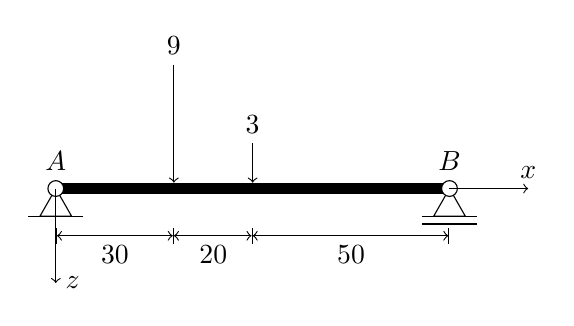
\begin{tikzpicture}
                \draw (-.2,-.25) -- (0,.1) -- (.2,-.25) -- cycle;
                \draw (-.35,-.25) -- (.35,-.25);
                \draw (4.8,-.25) -- (5,.1) -- (5.2,-.25) -- cycle;
                \draw (4.65,-.25) -- (5.35,-.25);
                \draw (4.65,-.35) -- (5.35,-.35);
                \fill (0,.025) rectangle (5,.175);
                \draw[fill=white] (0,.1) circle (1mm);
                \draw[fill=white] (5,.1) circle (1mm);
                \node[anchor=south] at (0,.2) {\(A\)};
                \node[anchor=south] at (5,.2) {\(B\)};
                \draw[->] (1.5,1.675) node[above] {\textbf{}\(9\sis{\kilo\newton}\)} -- (1.5,.175);
                \draw[->] (2.5,.675) node[above] {\(3\sis{\kilo\newton}\)} -- (2.5,.175);
                \draw[|<->|] (0,-.5) -- (1.5,-.5) node[midway,below] {\(30\sis{\centi\meter}\)};
                \draw[<->|] (1.5,-.5) -- (2.5,-.5) node[midway,below] {\(20\sis{\centi\meter}\)};
                \draw[<->|] (2.5,-.5) -- (5,-.5) node[midway,below] {\(50\sis{\centi\meter}\)};
                \draw[->] (0,.1) -- (0,-1.1) node[right] {\(z\)};
                \draw[->] (5,.1) -- (6,.1) node[above] {\(x\)};
            \end{tikzpicture}
            \quad
            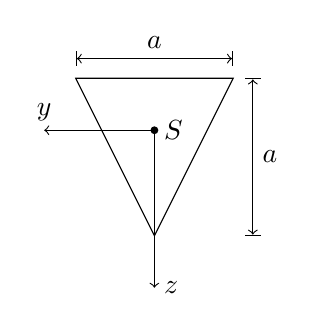
\begin{tikzpicture}
                \draw (0,1.1) -- (2,1.1) -- (1,-.9) -- cycle;
                \draw[|<->|] (0,1.35) -- (2,1.35) node[midway,above] {\(a\)};
                \draw[|<->|] (2.25,1.1) -- (2.25,-.9) node[midway,right] {\(a\)};
                \fill (1,.44) circle (.5mm) node[right] {\(S\)};
                \draw[->] (1,.44) -- (1,-1.56) node[right] {\(z\)};
                \draw[->] (1,.44) -- (-.4,.44) node[above] {\(y\)};
            \end{tikzpicture}
        \end{center}
        \begin{enumerate}
            \item Ermitteln Sie die Verläufe der Normal- und Querkraft sowie des Biegemomentes und deren Extremwerte.
            \item Berechnen Sie für die maximal zulässige Biegespannung \(\sigma_{\text{max}} = 14\sis{\kilo\newton\per\centi\meter\squared}\) das notwendige Querschnittsmaß \(a\).
            \item Mit dem berechneten Maß \(a\) ist dann die Biegespannungsverteilung im am stärksten beanspruchten Querschnitt zu ermitteln.
        \end{enumerate}
    \end{problem}
    
    \subsection*{Lösung}
    \begin{enumerate}
        \item Aus dem Kräfte- und Momentgleichgewichten
        \begin{align*}
            \sum F_x: &\quad A_x + B_x = 0,\\
            \sum F_z: &\quad A_z + B_z - 9\sis{\kilo\newton} - 3\sis{\kilo\newton} = 0,\\
            \sum M_A: &\quad \parentheses*{30\sis{\centi\meter} + 20\sis{\centi\meter} + 50\sis{\centi\meter}}B_z - 30\sis{\centi\meter} \cdot 9\sis{\kilo\newton} - \parentheses*{30\sis{\centi\meter} + 20\sis{\centi\meter}} \cdot 3\sis{\kilo\newton}
        \end{align*}
        folgen mit \(B_x = 0\) (Loslager) die Auflagerreaktionen
        \[
            A_x = 0, \quad A_z = 7,8\sis{\kilo\newton}, \quad B_x = 0, \quad B_z = 4,2\sis{\kilo\newton}.
        \]
        Für den ersten Abschnitt (\(0 \le x < 30\sis{\centi\meter}\)) ergeben sich die Kraft- und Momentverläufe zu
        \begin{align*}
            \sum F_x: &\quad N_1\parentheses*{x} = 0,\\
            \sum F_z: &\quad Q_1\parentheses*{x} = A_z = 7,8\sis{\kilo\newton},\\
            \sum M_S: &\quad M_1\parentheses*{x} = A_z x = 7,8\sis{\kilo\newton} \cdot x
        \end{align*}
        und für die lokalen Extremwerte folgt
        \begin{align*}
            N_{1, \text{min}} &= 0, & Q_{1, \text{min}} &= 7,8\sis{\kilo\newton}, & M_{1, \text{min}} &= 0,\\
            N_{1, \text{max}} &= 0, & Q_{1, \text{max}} &= 7,8\sis{\kilo\newton}, & M_{1, \text{max}} &= 2340\sis{\newton\meter}.
        \end{align*}
        Für den zweiten Abschnitt (\(30\sis{\centi\meter} \le x < 50\sis{\centi\meter}\)) ergeben sich die Kraft- und Momentverläufe zu
        \begin{align*}
            \sum F_x: &\quad N_2\parentheses*{x} = 0,\\
            \sum F_z: &\quad Q_2\parentheses*{x} = A_z - 9\sis{\kilo\newton} = -1,2\sis{\kilo\newton},\\
            \sum M_S: &\quad M_2\parentheses*{x} = A_z x - 9\sis{\kilo\newton} \cdot \parentheses*{x - 30\sis{\centi\meter}} = -1,2\sis{\kilo\newton} \cdot x + 2700\sis{\newton\meter}
        \end{align*}
        und für die lokalen Extremwerte folgt
        \begin{align*}
            N_{2, \text{min}} &= 0, & Q_{2, \text{min}} &= -1,2\sis{\kilo\newton}, & M_{2, \text{min}} &= 2100\sis{\newton\meter},\\
            N_{2, \text{max}} &= 0, & Q_{2, \text{max}} &= -1,2\sis{\kilo\newton}, & M_{2, \text{max}} &= 2340\sis{\newton\meter}.
        \end{align*}
        Für den dritten Abschnitt (\(50\sis{\centi\meter} \le x < 100\sis{\centi\meter}\)) ergeben sich die Kraft- und Momentverläufe zu
        \begin{align*}
            \sum F_x: &\quad N_3\parentheses*{x} = 0,\\
            \sum F_z: &\quad Q_3\parentheses*{x} = -B_z = -4,2\sis{\kilo\newton},\\
            \sum M_S: &\quad M_3\parentheses*{x} = B_z \cdot \parentheses*{100\sis{\centi\meter} - x} = -4,2\sis{\kilo\newton} \cdot x + 4200\sis{\newton\meter}
        \end{align*}
        und für die lokalen Extremwerte folgt
        \begin{align*}
            N_{3, \text{min}} &= 0, & Q_{3, \text{min}} &= -4,2\sis{\kilo\newton}, & M_{3, \text{min}} &= 0,\\
            N_{3, \text{max}} &= 0, & Q_{3, \text{max}} &= -4,2\sis{\kilo\newton}, & M_{3, \text{max}} &= 2100\sis{\newton\meter}.
        \end{align*}
        Somit ergeben sich die globalen Extremwerte
        \begin{align*}
            N_{\text{min}} &= 0, & Q_{\text{min}} &= -4,2\sis{\kilo\newton}, & M_{\text{min}} &= 0,\\
            N_{\text{max}} &= 0, & Q_{\text{max}} &= 7,8\sis{\kilo\newton}, & M_{\text{max}} &= 2340\sis{\newton\meter}.
        \end{align*}
        \item Da der Schwerpunkt des Dreiecks \(\frac{1}{3}a\) unterhalb der oberen Kante liegt, folgt \(z_{\text{max}} = \frac{2}{3}a\) und mit dem Flächenträgheitsmoment
        \[
            I_y = \frac{bh^3}{36} = \frac{a^4}{36}
        \]
        folgt für das Widerstandsmoment
        \[
            W = \frac{I_y}{\absolute*{z_{\text{max}}}} = \frac{a^3}{24}.
        \]
        Das notwendige Querschnittsmaß \(a\) folgt aus der maximalen Biegespannung, welche sich aus dem maximalen Biegemoment ergibt.
        Daher folgt mit
        \[
            \absolute*{\sigma_{B, \text{max}}} = \absolute*{\sigma_{\text{zul.}}} = \frac{M_{\text{max}}}{W} = \frac{24 \cdot 2340\sis{\newton\meter}}{a^3}
        \]
        für das Querschnittsmaß \(a\)
        \[
            a = \sqrt[3]{\frac{24 \cdot 2340\sis{\newton\meter}}{\sigma_{\text{zul.}}}} = \sqrt[3]{\frac{56,16\sis{\kilo\newton\meter}}{140000\sis{\kilo\newton\per\meter\squared}}} = 7,375\sis{\centi\meter}.
        \]
        \item Aus Aufgabenteil a) wissen wir, dass \(M_{\text{max}}\) bei \(x = 30\sis{\centi\meter}\) auftritt.
        Aus der Formel für die Biegespannung
        \[
            \sigma_B\parentheses*{x, z} = \frac{M\parentheses*{x}}{W\parentheses*{z}} = \frac{M\parentheses*{x}}{I_y}z
        \]
        folgt für den gefragten Querschnitt bei \(x = 30\sis{\centi\meter}\) der lineare Biegespannungsverlauf
        \[
            \sigma_B\parentheses*{30\sis{\centi\meter}, z} = \frac{2340\sis{\newton\meter}}{I_y}z = \frac{84240\sis{\newton\meter}}{a^4}z
        \]
        mit den Extremalwerten an den Rändern
        \[
            \sigma_B\parentheses*{30\sis{\centi\meter}, -\frac{1}{3}a} = -7\sis{\kilo\newton\per\centi\meter\squared}, \quad \sigma_B\parentheses*{30\sis{\centi\meter}, \frac{2}{3}a} = 14\sis{\kilo\newton\per\centi\meter\squared}.
        \]
    \end{enumerate}
\end{document}